\chapter{Dynamic logic}
Until now we have studied static logics in whitch the output node it's always connected to gnd or $V_{DD}$ through a low impedance path.\\
Dynamic logics feature high impedance at the output and the information is stored in a capacitance.\\


\section{Static and dynamic proprieties}

This technology reduce the capacitances (both input and output) by using a single clocked pmos transistor (and a clocked nmos too)

\centering
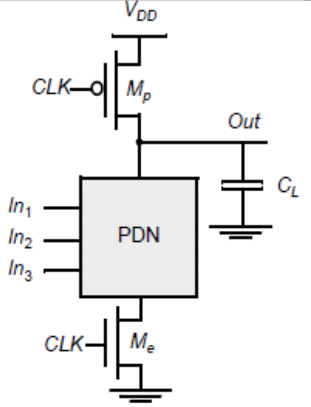
\includegraphics[width=0.35\textwidth]{C9_1.png}\\
\raggedright

This device has 2 phases: pre-charge and evaluation.\\
When CLK=0 we are in the pre-charge phase the pull-down network is disabled by the last nmos and the clocked pmos charge the output capacitance.\\
When CLK=1 we are in the evaluation phase the pull-down network is enabled and if the inputs are high than the output capacitance can be discharged. In order to the gate to work proprely during this phase the input signals can have only low to high transitions or they can remain stable (if they have a h-l commutation the output cannot change to high).\\
\vspace{5mm}
The logic function is implemented by the pull-down network that is the same of an FC-CMOS gate. The overall number of transistor is reduced at N+2 without losing the ratioless propriety. Reducing the number of transistors also the capacitance are reduced therefor we get an increase of speed.\\
\vspace{5mm}
Noise margins cannot be evaluated since we can't draw a characteristics but we can say that NMH$\simeq V_{DD}-V_{tp}$ and NML$\simeq V_{tn}$.\\
\vspace{5mm}
The positive aspects of this technology is that both input and output capacitance are smaller and we avoid any short circuit current with ideal clock signal.\\
However we have consider that we have another source of power dissipation that is the clock and that the switching activity is larger since p(1)=1 so 
\begin{equation}
\alpha_{sw}=p(0)
\end{equation}

\section{Issues in dynamic logic}
There are several issues that have to be take into account to verify that the circuit works proprely


\subsection{Leakage current}

\vspace{3mm}
\centering
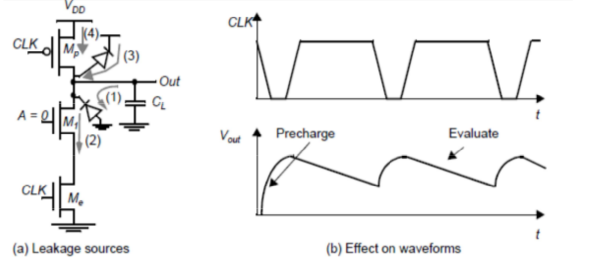
\includegraphics[width=0.5\textwidth]{C9_2.png}\\
\raggedright
\vspace{3mm}

If the clock frequency is very low sketching the output voltage, we can observe that it does not remain at $V_{DD}$ during the evaluation phase but slightly decreases. This effect is due to the leakage current.
This is a problem only at low frequency of the clock when the voltage across the capacitance can decrease more than $V_{DD}/2$.\\
\vspace{5mm}

We can use two solutions to avoid this drawback.\\
\tab I) Adopt a bleeder that keeps the output node at high level during the evaluation phase. But in this way we restore the ratioed problems so the transistor has to be correctly sized in order to be let the pull-down network dominate.\\
\tab II) Use a pmos transistor in feedback configuration that operates only if the output voltage is high. This is still a ratioed solution since if the output is high and the pull-down network is enabled the pmos has to be enought weak to let the nmos prevail and discharge the capacitance

\centering
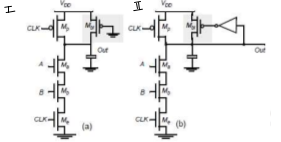
\includegraphics[width=0.45\textwidth]{C9_3.png}\\
\raggedright


\subsection{Charge sharing}
This is a problem of the inter-nodes parasitic capacitances that until now we've negleced.\\
Let's consider a 2 input NAND

\centering
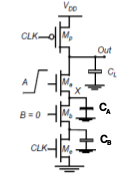
\includegraphics[width=0.25\textwidth]{C9_4.png}\\
\raggedright

If we are in the pre-charge phase and the input A toggles we have a charge sharing problem that varies the output voltage.\\
We can separate two cases large variation of the output or small variations.\\
\vspace{3mm}
For large variation of the output voltage ($\Delta V_{out}=V_{DD}-V_{out}\ge V_{tn} $) at the end the source of Ma will be the same as the output voltage at the end so we get that 
\begin{equation}
\Delta V_{out}=V_{DD}\frac{C_A}{C_L+C_A}
\end{equation}

\vspace{3mm}
For variations smaller than the nmos threshold the voltage at the source grows but cannot reach the output since the mos is shut off earlier.\\
In this case 
\begin{equation}
\Delta V_{out}=(V_{DD}-V_{tn})\frac{C_A}{C_L}
\end{equation}

\vspace{3mm}
The case change with the value of the ratio of the two capacitance; equating  the two equation to $V_{tn}$ we get that the limit is (considering also the body effect
\begin{equation}
\frac{C_A}{C_L}=\frac{V_{tn}}{V_{DD}-V_{tn}} = 0.38
\end{equation}
This means that $C_A$ has to be smaller than 0.38$C_L$.\\


\vspace{5mm}
The solution is to precharge also the internal node as in figure

\centering
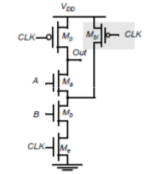
\includegraphics[width=0.15\textwidth]{C9_5.png}\\
\raggedright

\subsection{Capacitive coupling}

\centering
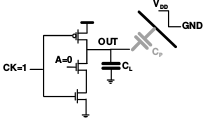
\includegraphics[width=0.35\textwidth]{C9_6.png}\\
\raggedright

High impedance node are very sensitive to interference and crosstalk so we have to be carefoul in the design of the overall circuit to do not put wires near the output of a dynamic gate in order to avoid interference and "parasitic" toggles due to a switch of the line.
The resulting voltage drop at the output is 
\begin{equation}
\Delta V_{out}=\frac{C_p}{C_L+C_p}V_{DD}
\end{equation}

\subsection{Clock feedthrough}
It's a particular type of clock feedthrough that can cause latch-up problems.\\


\section{Cascading dynamic gates}
The problem in cascading dynamic gates is that only a low to high transition is permitted during the evaluation phase (or a stable signal).\\
We can cascade dynamic gates in two different ways.

\subsection{Domino Logic}

\centering
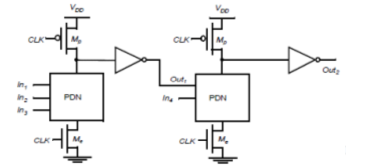
\includegraphics[width=0.35\textwidth]{C9_7.png}\\
\raggedright

During the pre-charge phase, the output of the dynamic logic is charged up to $V_{DD}$ while the inverter output is driven low. During the evaluation phase, the dynamic gate eventually discharges its output node and the output of the inverter transitions from 0 to 1. Otherwise, it remains low. This ensures that only transitions from 0 to 1 can happen in the evaluation phase.
In this way sequential logic gates are driven by low impendance device increasing the reliability.\\
The main drawback is that it's impossible to implement inverting functions in this way.\\
\vspace{5mm}
Alternative way is to use the unfooted logic (wihout the clocked nmos) or the Dual Rail Domino logic.\\

\centering
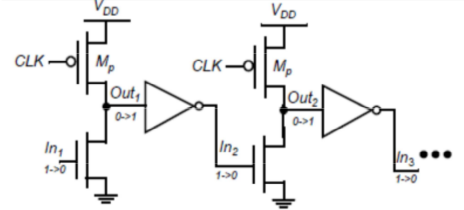
\includegraphics[width=0.35\textwidth]{C9_8.png}\\
\raggedright

\centering
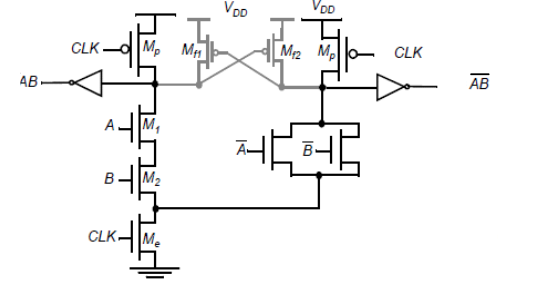
\includegraphics[width=0.35\textwidth]{C9_9.png}\\
\raggedright



\subsection{NP-CMOS dynamic}

\centering
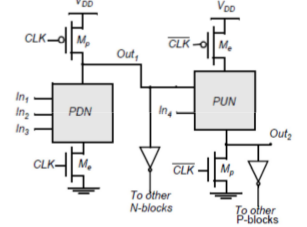
\includegraphics[width=0.35\textwidth]{C9_10.png}\\
\raggedright

The idea is to cascade n-type dynamics gate to p-type in order to have always the correct commutation during the evaluation phase (note that both type have simultaniously evaluation and precharge phase).\\




























































































































































